\documentclass{homework}
\usepackage{graphicx}

\title{ELEC400m Assignment 2}
\author{Matthew\ Sam}
\date{05/11/2022}

\begin{document}

\maketitle

\exercise

\large
PCA


I have also included my handwritten work for this question on the end of the pdf 



a)

Solving for the eigenvalues of X*transpose(X)
\begin{equation}
\begin{split}

X = \begin{bmatrix}
 1& 0 & 1 & 0\\ 
 1& 0 & 1 & 0\\ 
 1& 0 & 1 & 0
\end{bmatrix}
\par

X^{T} = \begin{bmatrix}
 1& 1 & 1\\ 
 0& 0 & 0\\ 
 1& 1 & 1\\
 0&0&0
\end{bmatrix}
\par


X*X^{T} =  \begin{bmatrix}
 1& 0 & 1 & 0\\ 
 1& 0 & 1 & 0\\ 
 1& 0 & 1 & 0
\end{bmatrix}
\begin{bmatrix}
 1& 1 & 1\\ 
 0& 0 & 0\\ 
 1& 1 & 1\\
 0&0&0
\end{bmatrix}
= \begin{bmatrix}
2 & 2 & 2\\ 
2 & 2 & 2\\ 
2 & 2 & 2
\end{bmatrix}

\newline
\end{split}
\end{equation}

solving for \[ det(XX^{T}-\lambda I) = 0 \] yields \[ 6\lambda^{2}-\lambda^{3} = 0 \]

solving for this equation gives us our eigenvalues:

\[
\lambda_{1}=6\]
\[ 
\lambda_{2}=0\]
\[ 
\lambda_{3}=0\]

b)

Our first principle component is \(\lambda_{1}\) and our first principle axis will be the eigenvector found using \(\lambda_{1}\)
\newline
by substituting \(\lambda_{1}\) into \( det(XX^{T}-\lambda I) = 0 \) we get the matrix:

\[
\begin{bmatrix}
-4 & 2 & 2 & 0\\ 
 2& -4 & 2 & 0\\ 
 2& 2 & -4 & 0
\end{bmatrix}
\]

then by preforming row reduction we can acquire out eigenvector/principle axis of:
\[
\bar{v_{1}} = <1,1,1>
\]


c)

By performing the same steps done in part a) we find that \(X^{'}X^{'T}\) ends up being the same as \(XX^{T}\). This means that if we would end up with identical principle components and axis. This is beneficial because it means that reordering of data does not change the results.
\newpage
\exercise*
a)

\centering
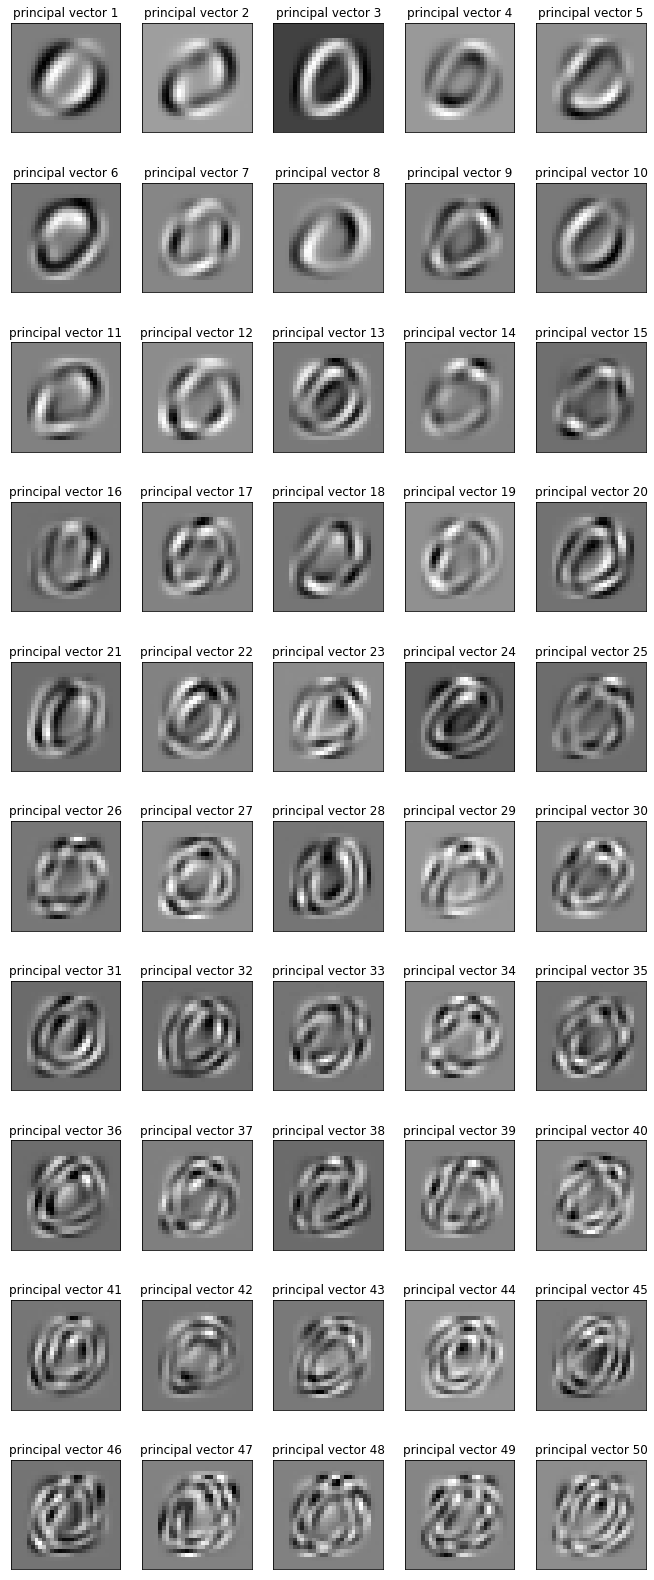
\includegraphics[width=250]{PCA_result.png}

\caption{figure 1: PCA results}

\raggedright

\exercise*
a)

\centering
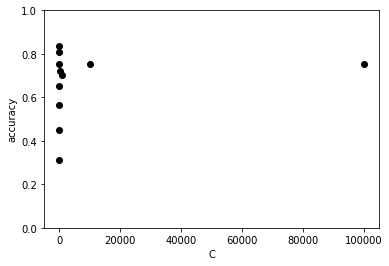
\includegraphics[width=250]{2a.png}
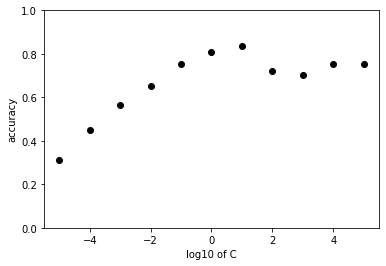
\includegraphics[width=250]{2a2.png}

\caption{figure 1: LinearSVC results}

\raggedright


b)

\centering
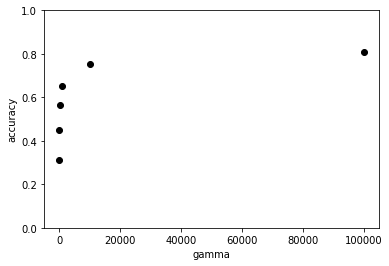
\includegraphics[width=250]{2b.png}
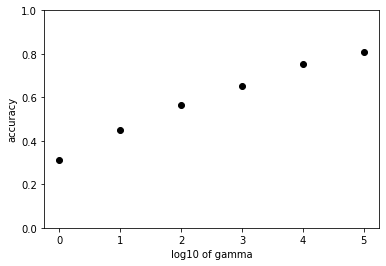
\includegraphics[width=250]{2b2.png}

\caption{figure 1: SVC results}

\raggedright



c)

\centering
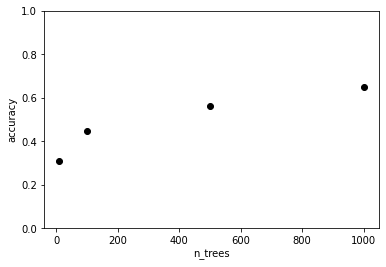
\includegraphics[width=250]{2c.png}
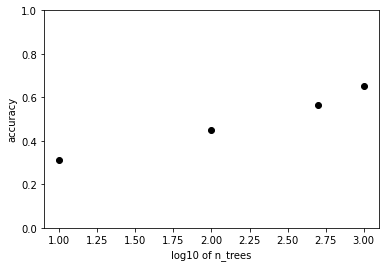
\includegraphics[width=250]{2c2.png}

\caption{figure 1: random forest results}

\raggedright


d)

The reported optimal hyper-parameter values found were:
\newline


C=10.0 for Linear SVC with a corresponding accuracy score of 0.836
\newline


gamma=0.1 for SVC with a corresponding accuracy score of 0.81
\newline


n=1000 RandomForest with a corresponding accuracy score of 0.81
\newline


the reported values for the hyper-parameters match those that can be seen visually in the graphs in part a-c.


\end{document}
